\chapter{مقدمه‌ای بر دستگاه عصبی}
\section{مقدمه}
در این فصل به مروری کوتاه بر اجزای تشکیل دهنده‌ی دستگاه عصبی\footnote{\lr{Nervous System}} می‌پردازیم که بواقع با داشتن مسئولیت ادراک و کنترل دیگر اعضای بدن، می‌توان آن را مهمترین بخش از بدن موجودات زنده نامید. 
دستگاه عصبی تحت یک فرآیند فرگشت\footnote{\lr{Evolutionary Process}} به چنان سطحی از تکامل رسیده است که به راستی آن را پیچیده‌ترین عنصر در جهان هستی معرفی می‌کنند. از خواص ویژه‌ی دستگاه عصبی می‌توان به تاثیر‌پذیری از محرک‌های خارجی، ایجاد یک جریان عصبی که نمایانگر تاثیر محرک می‌باشد و هدایت جریان عصبی از یک نقطه از دستگاه به نقاط دیگر نام برد.

دستگاه عصبی را می‌توان در سطوح مختلف، متناسب با اندازه و پیچیدگی عملکردشان، بررسی کرد. 
نورون\footnote{\lr{Neuron}} اصلی‌ترین یاخته‌ی عصبی است و وظیفه‌ی انتقال اطلاعات عصبی را برعهده دارد. هر نورون تنها یک آکسون\footnote{\lr{Axon}} و چندین دارینه\footnote{\lr{Dendrite}} دارد که از طریق دارینه‌ها سیگنال را از نورون پیش‌سیناپسی دریافت و بعد از تجمیع در جسم یاخته‌ای\footnote{\lr{Soma}} از طریق آکسون به نورون پس‌سیناپسی منتقل می‌کند. سیگنالی که از طریق آکسون مخابره می‌گردد منجر به ترشح یکسری مواد شیمیایی خاص، تحت عنوان پیام‌رسان عصبی\footnote{\lr{Neurotransmitter}}، از طریق اتصال سیناپسی می‌شود که می‌تواند به برانگیختن\footnote{\lr{Excitation}} یا مهار\footnote{\lr{Inhibition}} نورون‌های دریافت کننده‌ی سیگنال منتهی شود. 

\begin{figure}
\centering
{\footnotesize
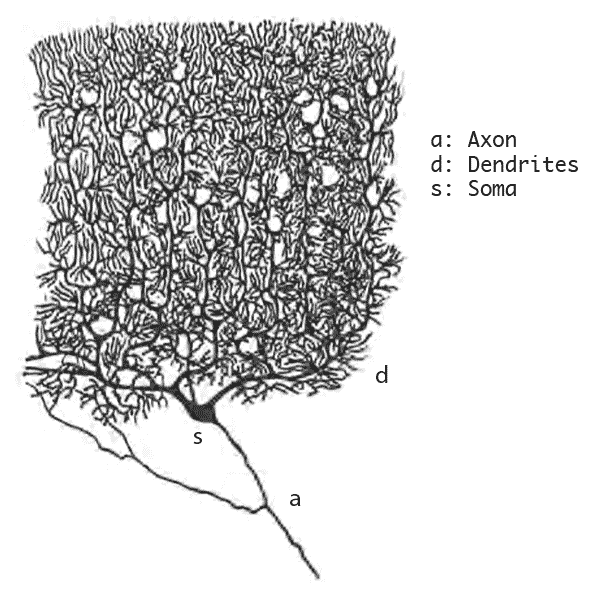
\includegraphics[height=5.5cm, width=7cm]{1_neuron}
\caption{سوما، آکسون و دارینه‌ها}
\label{fig:1_neuron}
}
\end{figure}

\section{فیزیولوژی نورون}
همانگونه که گفته شد، نورون‌ها واحدهای سازنده‌ی سیستم عصبی می‌باشند. تعداد نورون‌ها در گونه‌های مختلف جانوری متفاوت است و از چند نورون در کرم، ۱۰۰ هزار نورون در مگس و ۷۵ میلیون نورون در مغز موش متغیر است. در مغز انسان حدود ۱۰۰ بیلیون سلول عصبی یا نورون وجود دارد که هر کدام به طور متوسط به ۱۰ هزار نورون دیگر متصل است. پس در مجموع چیزی در حدود یک تریلیون اتصال سیناپسی وجود دارد.

اغلب نورون‌ها ساختاری به نسبت مشابه دارند اما با این حال عملکرد و وظایف نورون‌ها می‌تواند بسیار متفاوت باشد. نورون‌ها در اندازه، شکل و موقعیت قرارگیری با یکدیگر تفاوت دارند که تمام اینها وابسته به کاری است که یک نورون باید به طور مشخص انجام دهد. موارد مختلفی در تمایز نورون‌ها از دیگر سلول‌ها نقش دارد؛ از جمله اینکه آنها تقسیم نمی‌شوند و در طول عمر باقی مانده و نمی‌توانند جایگزین شوند. با وجود اینکه تقریبا تمام سلول‌های بدن به صورت شیمیایی با هم ارتباط دارند، می‌توان با اغماض گفت که تنها سلول‌های عصبی هستند که ارتباط الکتریکی دارند. مزیت ارتباط الکتروشیمیایی سرعت بسیار بالای آن است که امکان عمل و عکس‌العمل سریع را فراهم می‌کند.

عموما نورون به صورت سلولی مشاهده می‌شود که از دو قطب «ورودی» و «خروجی» تشکیل شده است. نورون‌ها از محیط خارج از خود، سیگنال‌هایی تحت قالب پالس‌های شیمیایی دریافت می‌کنند که منجر به تغییر حالت جاری آنها می‌شود. اگر تحت تاثیر این محرک‌های خارجی، شرایط بخصوصی در نورون برآورده شود، در مقابل سیگنالی از نورون به سمت خارج (سلول‌های عصبی یا ماهیچه‌ای) هدایت می‌شود. در ادامه با ساز و کار این مکانیسم و بخش‌های تشکیل دهنده‌ی نورون آشنا خواهیم شد.

\subsection{جسم سلولی (سوما)}
بخش هسته‌دار نورون، جسم سلولی یا سوما خوانده می‌شود. شکل و اندازه‌ی جسم سلولی در نورون‌های مختلف متفاوت بوده و به اشکال مدور، بیضی، هرمی، ذوزنقه‌ای و ستاره‌ای مشاهده شده است. قطر جسم سلولی نیز از چند میکرون تا چند صد میکرون می‌تواند متفاوت باشد. نورون بدون سوما وجود ندارد، اما به طور استثنا نورون‌هایی داریم که دارینه یا آکسون ندارند. جسم سلولی نورون را پریکاریون\footnote{\lr{Perikaryon}} نیز می‌نامند و به واقع کارخانه‌ی نورون محسوب می‌گردد زیرا پروتئین‌های لازم برای بخش‌های مختلف سلول توسط آن تولید می‌شود. سیتوپلاسم\footnote{\lr{Cytoplasm}} و هسته\footnote{\lr{Nucleus}} اجزای تشکیل دهنده‌ی سوما می‌باشند.

سیتوپلاسم سلول‌های عصبی را نوروپلاسم\footnote{\lr{Neuroplasm}} می‌گویند که شامل شبکه‌ی آندوپلاسمی\footnote{\lr{Endoplasmic Reticulum}}، میتوکندری\footnote{\lr{Mitochondria}}، دستگاه گلژی\footnote{\lr{Golgi Apparatus}} و دانه‌های لیزوزوم\footnote{\lr{Lysosome}} بوده و وظایفی از جمله پروتئین‌سازی، فراهم کردن انرژی لازم برای سلول، غشا‌سازی و بسته‌بندی ترشحات نورونی را دارد. 

هسته اما شاید مهمترین بخش سوما در نورون باشد. هسته‌ی نورون، معمار و بایگان سلول قلمداد می‌شود. به عنوان بایگان، شامل ژن‌های تشکیل دهنده‌ی \lr{DNA}ای است که تاریخچه سلول را در خود نگه داشته و اطلاعات مبنای ساخت پروتئین‌های مشخصه آن سلول را تعیین می‌کند. 
به عنوان معمار، RNA را از روی DNA سنتز کرده و از طریق حفره‌ها به سیتوپلاسم می‌فرستد تا برای سنتز پروتئین استفاده گردد.

\subsection{غشای نورونی و کانال‌های یونی}
به اتم‌هایی که بار الکتریکی داشته باشند یون گفته می‌شود. این بار می‌تواند مثبت یا منفی باشد و بسته به آن، بین یون‌ها رانش و ربایش بوقوع می‌پیوندد. در خارج از غشای نورون‌ها، یونهای مختلف به وفور یافت می‌شود که اهم آنها عبارت است از سدیم ($NA^+$)، پتاسیم ($K^+$)، کلسیم ($Ca^{++}$) و کلرید ($Cl^-$). غشای نورون که از چربی تشکیل شده است مانع از شار آزاد یون‌ها شده و بدین ترتیب داخل نورون عموما شاهد اختلاف پتانسیلی با خارج آن است. با این حال یکسری کانال یونی روی سطح غشا وجود دارد که کنترل جریان یونها به داخل و خارج نورون را میسر می‌سازند. نورون‌ها همیشه به دنبال رساندن این اختلاف پتانسیل به یک مقدار تعادل\footnote{\lr{Equilibrium Point}} هستند. وقتی نورون در حالت استراحت است، داخل نورون نسبت به خارج آن مقدار منفی دارد. 

کانال‌های یونی می‌توانند به صورت انتخابی بعضی از یون‌ها را به داخل یا خارج راه بدهند. در حالت استراحت، یون‌های پتاسیم به راحتی از غشا عبور می‌کنند اما یون‌های کلرید و سدیم به سختی امکان عبور دارند. برخی از کانال‌ها صرفا بار مثبت، بعضی فقط بار منفی و برخی هم هر دو را برای سلول کنترل می‌کنند. بر اساس نوع کنترل، درگاهها به دسته‌های زیر تقسیم‌بندی شده‌اند:

\begin{itemize}
\item \textbf{درگاه ولتاژی\footnote{\lr{Voltage-Sensitive}}:} این نوع درگاه تنها به اختلاف پتانسیل غشای نورون پاسخگو می‌باشد و بسته به اختلاف پتانسیل در هر لحظه، میزان عبور یون‌ها را کنترل می‌کند تا اختلاف پتانسیل به نقطه‌ی تعادل برسد.
\item \textbf{درگاه شیمیایی\footnote{\lr{Ligand-Gated}}:} این کانال‌ها توسط لیگاند‌ها کنترل شده و در صورت برخورد با مواد شیمیایی خاصی، باز می‌شوند. این مواد شیمیایی ممکن است از طریق سلول‌های دیگر یا ترشح غدد درون‌ریز به نورون برسند.
\item \textbf{درگاه مکانیکی\footnote{\lr{Mechanically Gated}}:} در پاسخ به تغییر شکل فیزیکی در گیرنده‌های حسی مانند لمس یا فشار تغییر حالت می‌دهند.

خواهیم دید که شرایط خاصی برای نورون رخ می‌دهد که اختلاف پتانسیل نورون را بیش از اندازه افزایش می‌دهد. در این صورت درگاه‌های ولتاژی برای رهایی از این وضعیت، خیلی سریع اقدام به باز و بسته شدن می‌کنند که به موجب آن یک شوک الکتروشیمیایی در سراسر سلول انتشار می‌یابد. این شوک که به آن ضربه یا اسپایک\footnote{\lr{Spike}} گفته می‌شود به موجب وجود اتصالات نورونی، به سلول‌های عصبی دیگر نیز از طریق درگاه‌های شیمیایی انتقال پیدا می‌کند. 

\end{itemize}

\subsection{دارینه}
اکثر نورون‌ها یک بخش مشابه درخت دارند که به آن دارینه اطلاق می‌شود. مسئولیت دارینه دریافت اطلاعات از دیگر نورون‌ها است. دارینه‌ها به صورت زوائد متعدد، کوتاه و شاخه‌شاخه‌ای که از بدنه‌ی سلول گسترش یافته‌اند پیدا می‌شوند. در درون دارنیه‌ها، میتوکندری، شبکه آندوپلاسمی، ریبوزوم‌ها و سایر ضمائم سیتوپلاسمی نورون‌ها یافت می‌شود. سطح خارجی دارینه‌ها دارای گیرنده‌های غشائی است که اطلاعات را از نورون‌های دیگر دریافت می‌کند.

\subsection{آکسون}
علاوه بر زوائد کوتاهی که از پریکاریون خارج شده و دارینه نام داشتند، زائده‌ی بلندی با نام آکسون یا آسه خارج می‌شود. طول بلند این رشته امکان انتقال سریع سیگنال‌ها به فواصل بیشتر را می‌دهد. آکسون که می‌توان آن را به عنوان خروجی نورون در نظر گرفت، می‌تواند ضربه‌ها را به مقاصدی به کوتاهی ۰/۱ میلی‌متر یا به بلندی ۲ متر برساند. 

آکسون‌ها بر حسب میلین\footnote{\lr{Myelin}} بودن یا نبودن به دو دسته تقسیم می‌شوند. میلین یک لایه‌ی چربی است که آکسون را پوشانده و با عایق کردن آن و افزایش نارسانایی، سرعت انتقال پیام‌های الکتریکی در طول آکسون را افزایش می‌دهد. با این حال همه‌ی درازای آکسون از میلین پوشانده نشده و در فواصل برابر بخش‌هایی با نام گره رانویه\footnote{\lr{Nodes of Ranvier}} وجود دارند که پوشش میلین ندارند. گره‌های رانویه باعث می‌شوند که بار الکتریکی در نواحی بدون میلین القا شود و به جای اینکه بار الکتریکی کل مسیر آکسون را بپیماید، به صورت القایی نواحی آزاد را عبور کرده و انقال سیگنال با سرعت به مراتب بالاتری صورت پذیرد. میلین در دستگاه اعصاب پیرامونی\footnote{\lr{Peripheral Nervous System}} بوسیله‌ی سلول‌های شوآن\footnote{\lr{Schwann Cells}} و در دستگاه اعصاب مرکزی\footnote{\lr{Central Nervous System}} توسط یک نوع بافت همبند عصبی به نام اولیگودندروگلیا\footnote{\lr{Oligodendrocyte}}  تشکیل می‌شود. 

\subsection{سیناپس}
سیناپس\footnote{\lr{Synapse}} یا همایه، یک ساختار در پایانه‌ی آکسون یک نورون (پیش‌سیناپسی) است که از طریق آن سیگنال به دارینه‌ی یک نورون دیگر (پس‌سیناپسی) منتقل می‌گردد. در اثر سیگنال رسیده از طریق سیناپس، نورون پس‌سیناپسی می‌تواند برانگیخته (افزایش اختلاف پتانسیل) یا مهار(کاهش اختلاف پتانسیل) شود که به نوعی نمود پردازش اطلاعات در مغز است. 

سیناپس‌ها محل نمود شکل‌پذیری عصبی\footnote{\lr{Neuroplasticity}} و یادگیری هستند. به عبارتی خواص فیزیکی و شیمیایی سیناپس که شدت و قدرت سیگنال ارسال شده به نورون پس‌سیناپسی را مشخص می‌کند امکان تغییر دارد. این تغییرات ممکن است باعث کاهش یا افزایش پتانسیل القایی در نورون شده و به موجب آن فرکانس ضربه‌ها در نورون پس‌سیناپسی کمتر یا بیشتر شود. در واقع طبق نظر محققان علوم اعصاب، عمده‌ی یادگیری\footnote{\lr{Learning}} مغز به جهت تنظیم «اثر\footnote{\lr{Synaptic Efficacy}}» ساختار سیناپسی (یا «وزن» در ادبیات علوم اعصاب محاسباتی) صورت می‌گیرد. 

سیناپس‌ها می‌توانند در دو نوع دسته‌بندی گردند: الکتریکی و شیمیایی که با اینکه تعداد سیناپس الکتریکی کمتر است، ولی این نوع سیناپس در هر سیستم عصبی یافت می‌شود و اجازه‌ی جریان مستقیم و منفعل الکتریکی را می‌دهد.

\begin{itemize}
\item
\textbf{سیناپس الکتریکی:} در این نوع سیناپس، پایانه‌های پیش‌سیناپسی مستقیما به پایانه‌های پس‌سیناپسی متصل هستند. یون‌ها و مولکول‌های کوچک عبور داده شده و در نتیجه تغییرات الکتریکی تقریبا بلافاصله به نورون پس‌سیناپسی منتقل می‌گردد. یون‌ها به طور کلی به هر دو جهت این اتصالات می‌توانند جریان داشته باشند. با این وجود، اتصالات الکتریکی که تنها در یک جهت انتقال صورت دهند وجود دارد، به این سیناپس‌ها عموما اتصالات یکسوساز\footnote{\lr{Rectifying Junctions}} می‌گویند که استفاده آنها در همزمان‌سازی\footnote{\lr{Synchronization}} ضربه‌های نورون‌ها می‌باشد. 
\item
\textbf{سیناپس شیمیایی:}
این اتصالات پیچیده‌تر بوده و فاصله‌ی بین پایانه‌های پیش و پس‌سیناپسی به مراتب بزرگتر است. همچنین انتقال نه به صورت الکتریکی، بلکه به صورت شیمیایی و به وسیله‌ی پیام‌رسان‌های عصبی است. این مواد شیمیایی در کیسه‌هایی موسوم به کیسه‌های سیناپسی\footnote{\lr{Synaptic Vesicles}} در محل سیناپس‌های شیمیایی قرار دارند، با برخورد ضربه‌های آتش شده از نورون پیش‌سیناپسی به آنها، کیسه‌ها پاره شده و مواد داخل آنها آزاد می‌شود. حال اگر در آن محل، دریچه‌ای باشد که با ماده‌ی آزاد شده باز گردد، نورون پس‌سیناپسی از ضربه‌ی دریافت شده متاثر می‌شود. انواع مختلف این پیام‌رسان‌ها شناسایی شده‌اند که بسته به نوع آن (اسید‌آمینه، پپتید و مونو آمین)، شدت و اثر تقسیم‌بندی شده‌اند.
\end{itemize}

\section{انواع نورون}
همانگونه که گفته شد، با وجود شباهت‌های ساز و کار نورون‌ها، انواع مختلفی از نظر شکل و اندازه در بخش‌های مختلف دستگاه عصبی و گونه‌های مختلف جانوری شناسایی شده‌اند. نورون‌ها را می‌توان به طور کلی در سه دسته‌ی ذیل قرار داد:

\begin{itemize}
\item
\textbf{نورون تک‌قطبی\footnote{\lr{Unipolar}}:}
این گونه از نورون‌ها صرفا یک دنباله (آکسون) دارند که از سوما گسترش پیدا می‌کند. این نورون‌ها می‌توانند بسته به محیط، شاخه داده و آکسون یا دارینه تشکیل دهند. این نورون‌ها بیشتر در حشرات یافت می‌شود که سوما در پیرامون مغز قرار گرفته و از نظر الکتریکی غیرفعال هستند. در این نورون‌ها، عموما یک رشته نئوریت\footnote{\lr{Neurite}} از سوما به مغز می‌رود که البته ممکن است به شاخه‌های فراوانی بیانجامد و اتصالات بسیار پیچیده‌ای با نئوریت‌های دیگر برقرار کند. 

\item
\textbf{نورون دوقطبی\footnote{\lr{Bipolar}}:}
این گونه از نورون‌ها دارای دو دنباله از سوما که یکی آکسون و دیگری دارینه است می‌باشد. این نورون‌ها عموما در عملکردهای حسی، مانند بویایی، شنوایی، لامسه و بینایی دیده می‌شوند. مثال معمول آن، نورون‌های دوقطبی در شبکیه‌ی چشم یا فراوانی آنها در مسیر وابران سیگنال‌های حرکتی به عضله‌های حرکتی است. 

\item
\textbf{نورون چندقطبی\footnote{\lr{Multipolar}}:}
این نورون‌ها دارای یک آکسون و همچنین تعدادی دارینه هستند. اکثر نورون‌های مغز بخصوص نورون‌های حرکتی و نورون‌های میانی از این دسته هستند. 
\end{itemize}

\begin{figure}
\centering
{\footnotesize
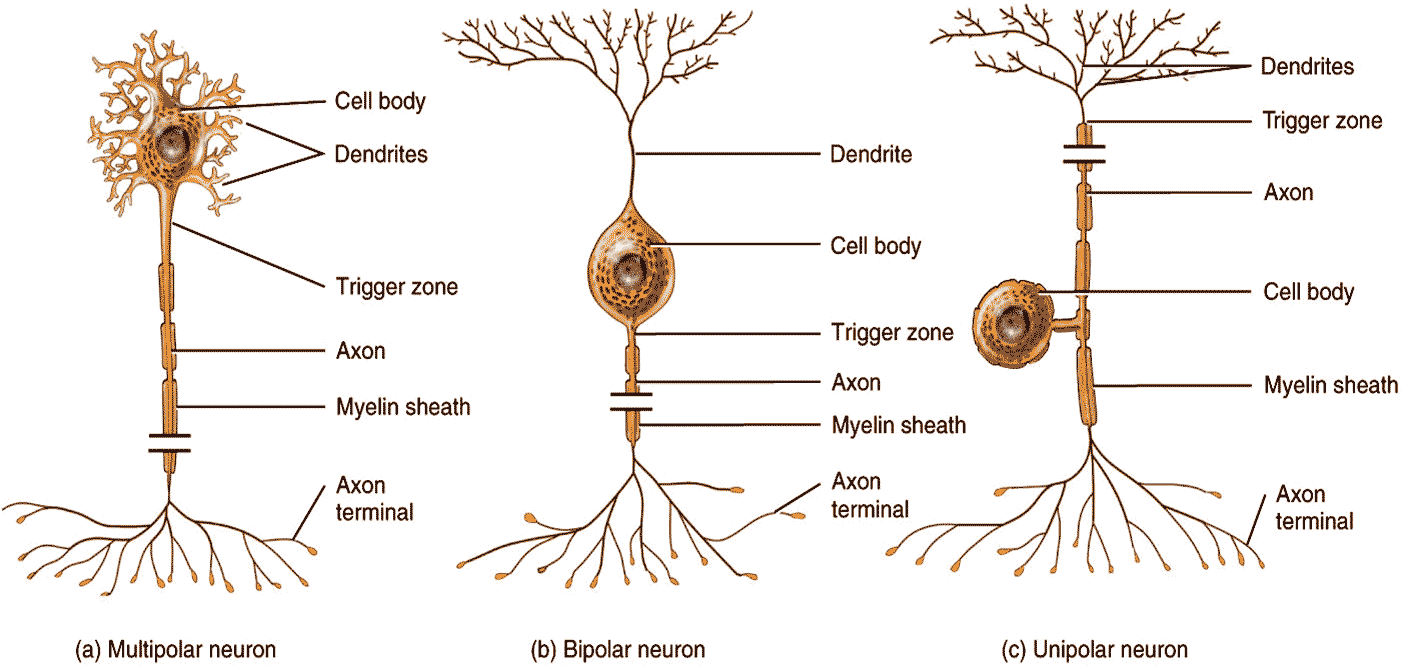
\includegraphics[height=7.5cm]{structural_neurons}
\caption{انواع نورون‌ها (تک‌قطبی، دوقطبی و چندقطبی)}
\label{fig:structural_neurons}
}
\end{figure}
\
\section{قانون هب}
نقش اساسی شکل‌پذیری\footnote{\lr{Plasticity}} در میانجیگری در اتصالات و فعالیت شبکه‌ی نورونی به صورت مفهومی در قالب نظریه‌ی هب\footnote{\lr{Hebbian theory}} بیان می‌شود. دونالد هب ادعا می‌نمود که از طریق مکانیسمی زیست‌فیزیکی، نورون‌ها در قالب رد عصبی\footnote{\lr{Engram}} سازمان پیدا می‌کنند؛ ساختارهای عصبی که امکان ذخیره‌ی رد حافظه را دارند. شاید نقل قول زیر\cite{hebb1949organization} از هب بهترین توضیح برای ادعای او باشد:

\textquote{
فرض کنید ماندگاری یا تکرار یک فعالیت ارتعاشی به القای تغییرات پایای سلولی منجر شود که به پایداری آن بیافزاید. زمانی که آکسون سلول A به اندازه‌ی کافی نزدیک باشد که به برانگیختن سلول B منجر شده و به صورت مداوم یا مکرر در آتش کردن آن نقش داشته باشد، یک فرآیند رشد یا تغییرات متابولیک در یک یا هر دو سلول رخ می‌دهد که در نتیجه‌ی آن بازده A به عنوان یکی از سلول‌های آتش کننده‌ی B افزایش می‌یابد. 
}

در علوم اعصاب به چنین اتصالی، «سیناپس هب» گفته می‌شود. این ادعا پشتیبانی تجربی قابل‌توجهی را کسب کرد، بخصوص با کشف تقویت بلند مدت\footnote{\lr{Long-term potentiation}} (LTP) و تضعیف بلند مدت\footnote{\lr{Long-term depression}} (LTD) که اولین بار در هیپوکمپوس\footnote{\lr{Hippocampus}} یافت شده\cite{bliss1973long} و بعدها در نواحی دیگری مانند آمیگدال\footnote{\lr{Amygdala}} و نئوقشر\footnote{\lr{Neocortex}} نیز مشاهده شد. در علوم شناختی و علوم اعصاب محاسباتی این طرح پیشنهادی تحت عنوان «قاعده‌ی هب» شناخته شده و الگوریتم‌های یادگیری برای تنظیم وزن‌های اتصالات برمبنای آن ارائه شده است.

\subsection{یادگیری وابسته به زمان ضربه}
یادگیری وابسته به زمان ضربه\footnote{\lr{Spike-timing dependent plasticity}} (STDP) یک مصداق مشخص از ادعای هب است که میزان تغییرات سیناپسی را به ترتیب زمانی پتانسل‌های عمل (ضربه‌ها) ربط می‌دهد. STDP اولین بار بواسطه‌ی مشاهدات تجربی لِوی و ستیوارد\cite{levy1983temporal} که منجر به مطالعات نظری گردید به منصه ظهور رسید. STDP در شکل کاملش توسط مارکرام و همکارانش\cite{markram1997regulation} در شبکه‌های قشری و به طور همزمان توسط بِل و همکارانش\cite{bell1997synaptic} در ساختار مخچه‌مانند ماهی الکتریکی تبیین شد. 

هم اکنون STDP در سیناپس‌های برانگیزاننده از گستره‌ی وسیعی از مدارات عصبی مانند قشر بینایی، هیپوکمپوس، هسته‌ی پشتی حلزونی\footnote{\lr{Dorsal cochlear nucleus}}، دستگاه بویایی ملخ و... مشاهده شده است. 

برجسته‌ترین مشخصه‌ی STDP در وابسته بودن تغییرات سیناپسی به ترتیب زمانی زوج‌های ضربه‌ی پیش و پس‌سیناپسی است. به استثنای مواردی مانند ساختار مخچه‌مانند ماهی الکتریکی، اکثر مشاهدات تجربی نشان داده‌اند که وقتی یک ضربه‌ی پیش‌سیناپسی مقدم بر ضربه‌ی پس‌سیناپسی می‌شود، سیناپس تقویت می‌شود و در مقابل وقتی ترتیب زمانی معکوس باشد، سیناپس تضعیف خواهد شد. از این جهت STDP بر رابطه‌ی علّی میان نورون‌ها می‌افزاید. این مشاهدات موجب شده تا مدل‌های مبتنی بر زوج STDP ارائه گردد که تغییرات سیناپسی را بر اساس فاصله‌ی زمانی بین زوج‌های ضربه‌ی پیش و سیناپسی بیان می‌کنند. این دسته از مدل‌ها توانایی ساماندهی عملکردی مدارات عصبی را داشته و رخدادهای بسیاری، به مانند تشکیل میدان‌های تاثیر\footnote{\lr{Formation of receptive fields}}، رشد میزان‌سازی جهت\footnote{\lr{Development of orientation tuning}} و گزینندگی مسیر\footnote{\lr{Direction selectivity}} در قشر بینایی، تشکیل سلول‌های مکان\footnote{\lr{Place cells}} در هیپوکمپوس و یادگیری دنباله‌های زمانی را توضیح می‌دهد. 

در فصول بعدی به ابعاد بیشتری از مکانیسم STDP پرداخته و سازوکار آن را با بیان مدل ریاضیاتی مطرح می‌کنیم.